\documentclass[border=0.2cm]{standalone}

\usepackage[utf8]{inputenc}
\usepackage[T1]{fontenc}

\usepackage{tgadventor}
\usepackage{tikz}
\usepackage{siunitx}

\usetikzlibrary{arrows}

\renewcommand*\familydefault{\sfdefault}

\begin{document}
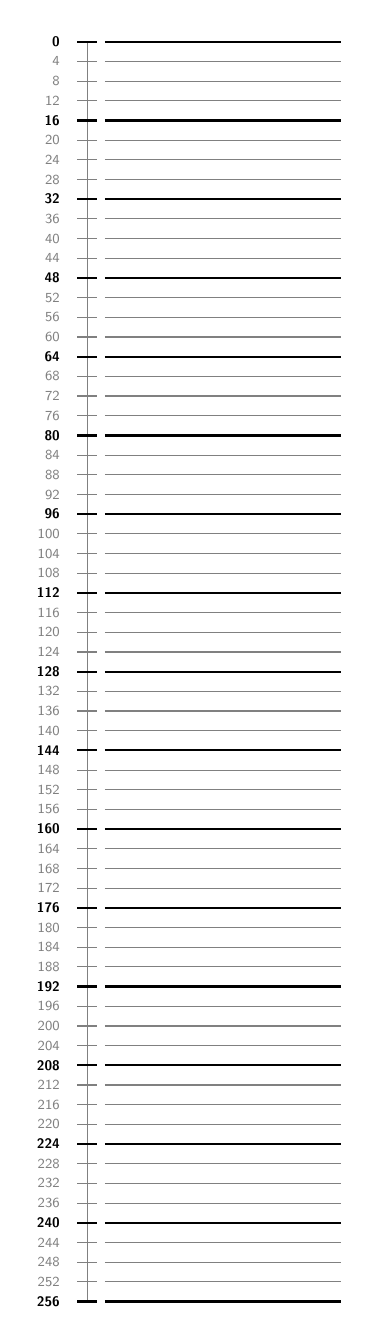
\begin{tikzpicture}[
    every node/.style={font=\normalfont\tiny},
]  
    \draw[gray] (.125, 0) -- (.125, -64*.25);
    \foreach \p in {0,...,64} {
        \pgfmathtruncatemacro{\num}{\p * 4}
        \pgfmathsetmacro{\highlight}{mod(\p,4)==0 ? 1 : 0}
        
        \ifnum \highlight=1 % compiles quicker online
            \draw (0, -\p*0.25) -- ++(.25, 0) [black,thick] ++(.1, 0) -- ++(3, 0);
            \draw (0, -\p*0.25) ++(-.1,0) node[black,anchor=east,font=\bfseries]{\tiny \num};
        \else
            \draw (0, -\p*0.25) -- ++(.25, 0) [gray,thin] ++(.1, 0) -- ++(3, 0);
            \draw (0, -\p*0.25) ++(-.1,0) node[gray,anchor=east]{\tiny \num};
        \fi 
    }
    
\end{tikzpicture}

\end{document}
